%!TEX root = ../thesis.tex
%*******************************************************************************
%****************************** Sixth Chapter *********************************
%*******************************************************************************

\chapter{An LMM framework for multivariate context-specific single cell eQTL mapping}
\label{chapter6}

% add abstract
As we have seen, \gls{scrnaseq} assays are now established and relatively cheap, which means that they can deployed at scale, across many individuals. 
As a result, eQTL mapping using single cell profiles, rather than bulk, to quantify gene expression, have arised (Chapter 3).\\

In particular, \gls{scrnaseq} can be used to first (unbiasedly) define discrete cell populations within an experiment, and then quantify expression within each cell population to map cell type- and condition-specific eQTL (Chapters 4, 5).
In alternative, the single cell transcriptome can be used to order cells along a developmental trajectory to map dynamic eQTL, where the effect of a genetic variant on expression is modulated by (pseudo)time (Chapter 4). \\

% It has been shown that single cell expression profiles can be used to estimate a number of discrete and continuous states for the cells considered,

Moreover, single cell expression profiles can be used to characterise cell-to-cell variation across a wide range of cell state dimensions,
including cell type and differentiation trajectory but also cell cycle phase, metabolic state,..
% available datasets (Chapters 4,5)\\
This means that within a single neatly contained experiment, one can have access to expression profiles for thousands of genes, across hundreds of individuals at single cell resolution, and cells can be unbiasedly annotated according to a number of factors. \\

This experimental set up calls for computational methods that would allow to jointly perform multi-context-specific eQTL, at single cell resolution.
Here, we propose scStructLMM, a method based on (Chapter 2).

\newpage

% \begin{Comment2}
% % \subsection{Contributions}
% \hspace{-3mm}\textbf{Contributions} I worked on this project in collaboration with Danilo Horta, Elissavet (Elsa) Kentepozidou, John Marioni and Oliver Stegle.
% In this project, I extended an existing model for identifying multivariate GxE interactions (StructLMM \cite{moore2019linear}) to the specific use case of scRNA-seq data.
% I worked out the necessary underlying maths necessary for the extension and helped re-writing the method in collaboration with Danilo. 
% The model is now a usable python package available here:
% Please also find the corresponding documentation here:

% Anna S.E. Cuomo, Danilo Horta, Elissavet Kentepozidou, Marc Jan Bonder, John C. Marioni, Oliver Stegle. 
% Title, 2020

% \end{Comment2}

% \newpage

\section{Introduction} 

As we have seen in the previous chapters, population-scale single-cell sequencing studies, which combine genotype information and single cell expression profiles across larger sets of individuals, have enabled the study of genetic effects on gene regulation at single-cell resolution (Chapter 3). 
Seminal studies have demonstrated the feasibility of mapping expression quantitative trait loci (eQTL) using single-cell readouts, thereby replicating conventional eQTL detected using bulk gene expression profiling \cite{cuomo2020single, van2018single}, detecting cell-type specific genetic effects \cite{van2018single} as well as identifying dynamic changes of regulatory effects across lineages or cellular differentiation \cite{cuomo2020single} (Chapter 4). 
Collectively, these efforts have demonstrated the potential of single-cell sequencing approaches to complement and generalise conventional eQTL mapping, elucidating context-specific regulation, which previously was limited to narrowly defined context such as cell types from sorted populations \cite{fairfax2012genetics} or external stimulation \cite{fairfax2014innate} (see section \ref{sec:eqtl}).\\

Despite this potential of single-cell genetics, appropriate analysis methods are only beginning to emerge. 
On the one hand existing multi-tissue eQTL methods designed for bulk profiling, which allow for mapping eQTL that are present in single tissues or combinations of tissues, remain applicable. 
For example, …\cite{flutre2013statistical, urbut2019flexible}.
However, these require to discretise single-cell profiles into cell types, which fails to fully leverage the advantages of single-cell readouts to detect complex gene-context interactions, in particular the ability to detect continuous changes and gradients. \\

Recently, methods to assess GxE using larger numbers of conditions have emerged in the context of population studies.
In particular, a recently proposed method called StructLMM (structured linear mixed model, described in section \ref{sec:struct_lmm}) allows for the robust joint analysis of GxE effect of multiple environmental variables \cite{moore2019linear}. \\


% population-scale cohorts that combine genotyping with single cell expression profiles have fostered interest to study the effect of common genetic variants on gene regulation at single cell resolution.\\

% It has already been demonstrated that single cell \gls{eqtl} mapping can be achieved, and that known \glspl{eqtl} previously identified using bulk expression can be replicated both in iPS cells and blood \cite{cuomo2020single,van2018single}.
% Additionally, the single cell resolution allows for the interrogation of interaction eQTL, where the strength of the genetic effect of eQTL is modulated by the cells’ types and states \cite{cuomo2020single}. 
% These kinds of studies can add a layer of interpretability of the role of genetic variants on gene expression regulation. 
% Analyses of eQTL context-specificity have been so far limited to a single state variable (e.g. cell type, \cite{fairfax2012genetics} or stimulation status,\cite{fairfax2014innate} ) and individual genetic variants.\\

% A recently proposed method called StructLMM (structured linear mixed model, described in 2.4.3) allows for the robust joint analysis of GxE effect of multiple environmental variables \cite{moore2019linear}.
% This model can be applied, with some care, to the mapping of interaction eQTL, where genes’ single cell expression profiles are the tested outcomes, and the cells’ states and types are the environmental variables. 
% The main limitation of StructLMM is that it does not allow to fully control for the intrinsic population structure of the tested samples [REF]. 
% When using single cell measurements, we are in practice dealing with genetically identical replicate observations for a donor. 
% The relatedness structure between samples (or cells in this context) is therefore non-trivial, as the cell measurements are not independent, as assumed by the model.\\

% without the previous paragraph this doesn't make any sense, rephrase
Here, we propose sc-StructLMM, an extension of the StructLMM model that builds on it while allowing control for confounding effects due to population structure, and is especially well suited for the mapping of multivariate single cell interaction eQTL. 
The model can handle hundreds of cell states and conditions, and it can be applied to large cohorts of hundreds of thousands of cells for hundreds of  individuals.

\begin{figure}[htbp]
\centering
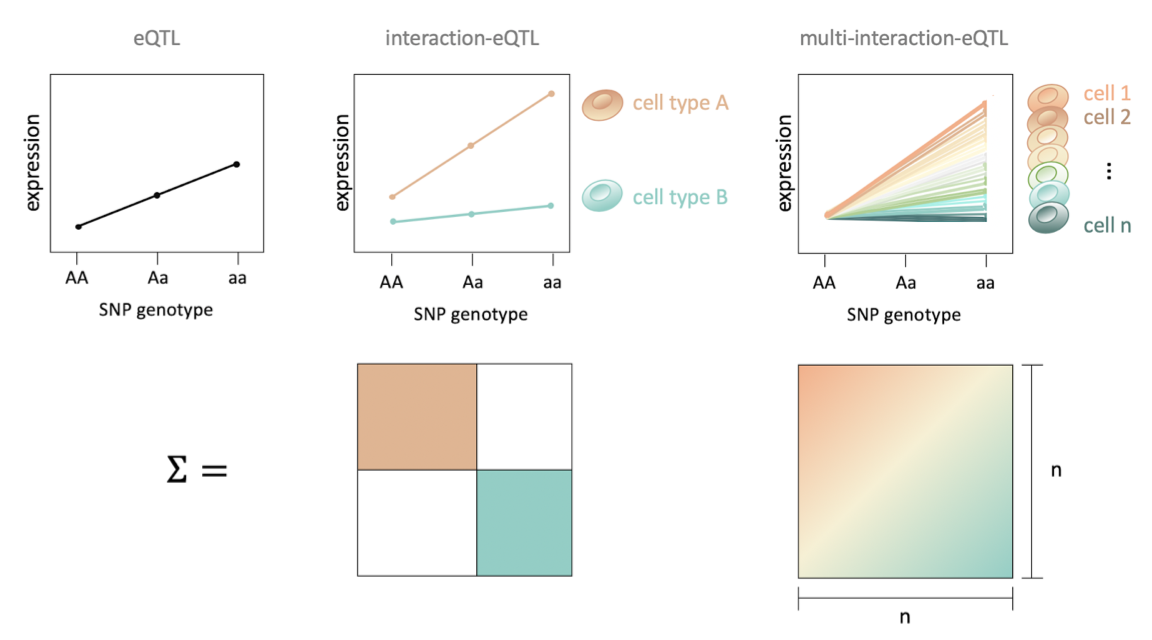
\includegraphics[width=15.5cm]{Chapter6/Fig/sc_structlmm_overview.png}
\caption[overview of model]{\textbf{overview of model}.\\
Overview.}
\label{fig:sc_structlmm_overview}
\end{figure}


\clearpage

\section{Model} 

As we have seen (Chapters 2-5), commonly used methods for eQTL mapping fit linear or linear mixed models (LMMs),  whereby a given variant is tested for association with expression changes of a target gene \cite{kilpinen2017common}. 
The effect size is assumed to be shared (persistent) across individuals, or alternatively a discrete group structure (e.g. tissues) can be accounted for \cite{fusi2012joint}. 
In contrast, scStructLMM borrows concepts from the previously described StructLMM model designed for global phenotypes \cite{moore2019linear}, whereby heterogeneity in effect sizes is defined by an environmental (context) covariance matrix, which can capture arbitrary sub-structure in cellular states. 
Specifically, scStructLMM generalises the previous approach by adding the ability to  account for two distinct sets of additive random effect components, which enables modelling of replicated measurements for the same donor, in particular the intrinsic repeat structure of single-cell eQTL studies where multiple cells are sampled form the same individual. 
The model can be cast as:

\begin{equation}\label{eq:scStructLMM}
 \mathbf{y} =  \mathbf{W}\boldsymbol{\alpha} + \mathbf{g}\beta_G + \mathbf{g} \odot \boldsymbol{\beta_{GxE}} + \mathbf{e} + \mathbf{u} + \boldsymbol{\psi}, 
\end{equation}

% where $\mathbf{e} \sim \mathcal{N}\mathbf{0},\sigma_e^2 \mathbf{E}\mathbf{E}^T)$, $\mathbf{u} \sim \mathcal{N}\mathbf{0},\sigma_g^2 \mathbf{G}\mathbf{G}^T)$ and $\boldsymbol{\psi} \sim \mathcal{N}\mathbf{0},\sigma_n^2 \mathbf{I_N})$.\\

where $\beta_G$ denotes the effect size of a conventional persistent genetic effect component, and $\boldsymbol{\beta_{GxE}}=[\beta_{GxE_1}, .. ,\beta_{GxE_N}]^T$ is a vector of per-cell effect sizes to account for heterogeneous genetic effects, which follows a multivariate normal distribution, $\boldsymbol{\beta_{GxE}} \sim \mathcal{N}(\mathbf{0},\sigma_{GxE}^2 \mathbf{E}\mathbf{E}^T)$. 
Depending on the functional form of the environmental covariance, this model can account for different types of G$\times$E, for example, both discrete and continuous cell states and types or donor-level environmental covariates. 
The same environmental covariance is also used to account for additive environmental effects, $\mathbf{e} \sim \mathcal{N}(\mathbf{0},\sigma_e^2 \mathbf{E}\mathbf{E}^T)$ \cite{moore2019linear}. 
Finally, additive global genetic effects are accounted for using a kinship matrix ($\mathbf{K}$) (calculated using PLINK \cite{purcell2007plink}, see section \ref{sec:linear_mixed_models}), such that
$\mathbf{u} \sim \mathcal{N}(\mathbf{0},\sigma_g^2 \mathbf{K})$,
% $\mathbf{u} \sim \mathcal{N}(\mathbf{0},\sigma_g^2 \mathbf{G}\mathbf{G}^T)$,
appropriately expanded to reflect the repeated structure of multiple cells derived from the same donors; finally the noise term is gaussian and i.i.d. $\boldsymbol{\psi} \sim \mathcal{N}(\mathbf{0},\sigma_n^2 \mathbf{I_N})$.\\

The test performed is equivalent to the StructLMM-int ($\sigma_{GxE}^2 > 0$).
To evaluate significance, we 
% Because we 
use Rao's Score test (see section \ref{sec:hypothesis_testing}), thus we only need to evaluate the MLE of the parameters 
% likelihood
under $H_0$:

\begin{equation}\label{eq:scStructLMM_H0}
 \mathbf{y}|H_0 =  \mathbf{W}\boldsymbol{\alpha} + \mathbf{g}\beta_G + \mathbf{e} + \mathbf{u} + \boldsymbol{\psi} 
\end{equation}

\begin{equation}\label{eq:scStructLMM_H0_MVN}
 \mathbf{y}|H_0 \sim \mathcal{N}( \mathbf{W}\boldsymbol{\alpha} + \mathbf{g}\beta_G, \sigma_e^2 \mathbf{E}\mathbf{E}^T + \sigma_g^2 \mathbf{G}\mathbf{G}^T+ \sigma_n^2 \mathbf{I} )
\end{equation}

Now, to be able to use the trick described in section 
% \ref{sec:fast_lmm},
% 2.3.3, 
we need to write the Covariance matrix in the form $\sigma^2(\mathbf{M}+\delta\mathbf{I})$ as in eq. \eqref{eq:fast_lmm_full_covariance}.
To do so, we introduce a weight parameter $\rho_1$ such that the covariance matrix of $\mathbf{y}$ under the null hypothesis, $\mathbf{K}_0 = Cov(\mathbf{y} | H_0)$ can be re-written as:

\begin{equation}
\begin{split}
    \mathbf{K}_0 = \sigma_e^2 \mathbf{E}\mathbf{E}^T + \sigma_g^2 \mathbf{G}\mathbf{G}^T+ \sigma_n^2 \mathbf{I} =\\
    \sigma_k^2[\rho_1\mathbf{E}\mathbf{E}^T + (1-\rho_1) \mathbf{G}\mathbf{G}^T] + \sigma_n^2 \mathbf{I} =\\ \sigma_k^2\{\boldsymbol{\Sigma}(\rho_1) + \delta_1 \mathbf{I}\},
\end{split}
\end{equation}

where $\sigma_k^2\rho_1 = \sigma_e^2$,
$\sigma_k^2(1-\rho_1) = \sigma_g^2$,
$\delta_1 = \sigma_n^2/\sigma_k^2$, and $\boldsymbol{\Sigma}(\rho_1) = \rho_1\mathbf{E}\mathbf{E}^T + (1-\rho_1) \mathbf{G}\mathbf{G}^T$.\\

I note that $\boldsymbol{\Sigma}$ only depends on $\rho_1$. 
To efficiently implement this, we perform a grid search over $\rho_1$ with as little as 10 possible values (from 0 to 1), thus only slowing down the original method by a factor of 10.

\section{Statistical testing}

To test for GxE interactions we apply the same strategy that is used in the StructLMM method, which in turn adopts the strategy described in Lippert et al \cite{lippert2011fast}.
% Rao et al \cite{rao1948large}.
I use this section to describe the key steps involved.
First, we define score-based test statistic Q as:

\begin{equation}\label{eq:Q}
    Q = \frac{1}{2}\mathbf{y}^T\mathbf{P}_0 \frac{\partial \mathbf{K}}{\partial \theta}\mathbf{P}_0 \mathbf{y}, 
\end{equation}

where $\mathbf{K}$ is the full covariance matrix (\eqref{eq:scStructLMM}):

\begin{equation}\label{eq:full_K_scStructLMM}
    \mathbf{K} = \sigma_{GxE}^2diag(\mathbf{g})\mathbf{E}\mathbf{E}^Tdiag(\mathbf{g}) +  \sigma_e^2 \mathbf{E}\mathbf{E}^T + \sigma_g^2 \mathbf{G}\mathbf{G}^T+ \sigma_n^2 \mathbf{I}
\end{equation}

and 

\begin{equation}
    \mathbf{P}_0 = \mathbf{K}_0^{-1}-\mathbf{K}_0^{-1}\mathbf{X}(\mathbf{X}^T\mathbf{K}_0^{-1}\mathbf{X})^{-1}\mathbf{X}^T\mathbf{K}_0^{-1}
\end{equation}

is a matrix that projects out the fixed effects \cite{lippert2011fast, lippert2014greater}.
In our case (eq. \eqref{eq:scStructLMM}), the fixed effects include covariates and the persistent effect of the variant tested: $\mathbf{X} = [\mathbf{W}, \mathbf{g}]$\\

Using \eqref{eq:full_K_scStructLMM} and considering the parameter $\theta = \sigma_{GxE}^2$, we can derive:

\begin{equation}
    \frac{\partial \mathbf{K}}{\partial \sigma_{GxE}^2} = diag(\mathbf{g})\mathbf{E}\mathbf{E}^Tdiag(\mathbf{g}).
\end{equation}

Next, let us define $\mathbf{K}_1 = diag(\mathbf{g})\mathbf{E}\mathbf{E}^Tdiag(\mathbf{g})$
and substituting in eq. \eqref{eq:Q}, we can write:

\begin{equation}
    Q = \frac{1}{2}\mathbf{y}^T\mathbf{P}_0 \mathbf{K}_1\mathbf{P}_0 \mathbf{y} 
\end{equation}

As in \eqref{eq:StructLMM-int_H1}, $H_1: \sigma_{GxE}^2>0$, noting that as a variance parameter, $\sigma_{GxE}^2$ can only take positive values.
As a result, the Score test statistic $Q$ does not follow the usual $\chi^2_i$ distribution (see eq. \eqref{eq:lagrange_multiplier_univariate}), but instead a mixture of  $\chi^2$ distributions.
I refer the donor specifically at the supplementary methods from \cite{lippert2014greater} for a proof.

\begin{equation}
    Q \sim \sum_i \lambda_i \chi^2_1 
\end{equation}

Where $\lambda_i$'s are the non-zero eigenvalues of $\frac{1}{2}\mathbf{P}_0^{\frac{T}{2}} \frac{\partial\mathbf{K}}{\partial \theta} \mathbf{P}_0^{\frac{1}{2}}$.\\

Now since the eigenvalues of $AA^T$ are the same as those of $A^TA$ (ref), we can re-arrange and compute $\lambda_i$'s as the eigenvalues of:

\begin{equation}
    \frac{1}{2}\frac{\partial\mathbf{K}}{\partial \theta}^{\frac{T}{2}} \mathbf{P}_0 \frac{\partial\mathbf{K}}{\partial \theta}^{\frac{1}{2}},
\end{equation}

instead.

To evaluate the significance of the score-best test statistic $Q$ we use the approach described in in SKAT \cite{wu2011rare}, thereby using the Davies exact method \cite{davies1980algorithm} to compute the corresponding p values, and switching to the modified moment matching approximation method \cite{liu2009new, lee2012optimal, duchesne2010computing} when this fails to converge.


% Various methods have been proposed to compute the tail probability of the mixture of 1-dof $\chi^2$ distributions. 
% For example, we can use the Davies method \cite{davies1980algorithm}, the moment‐matching‐based noncentral $\chi^2$ approximation method \cite{liu2009new, lee2012optimal}, or the saddlepoint approximation method \cite{kuonen1999miscellanea}. 
% The Davies methos is the most accurate but can be be computationally expensive.
% The moment-matching approximation is anti-conservative and could lead to inflated type I errors especially for small significance levels.
% SKAT: Davies + Liu
% SKATh: Davies + saddle
% \cite{wu2016efficient}

% \section{Definition of covariance matrix}

% E?

% PCs, MOFA, HVGs?
% transformation?
% normalization/scaling

\newpage

\section{Simulation data}

% First, we applied the model on simulated data.

Simulation experiments were used to show that scStructLMM is calibrated, and then to demonstrate the 
% power 
advantages of scStructLMM compared to other methods. 
% forthe interaction and association test (Section 2.3). 

In this section, I will first describe the data used for these experiments, the simulation procedure used to generate phenotypes and the methods used to assess calibration and statistical power. 
% I will then show calibration and power results for some general settings, followed by results for simulation experiments that explicitly examine the effect of certain environmental properties.

\subsection{Simulation strategy}

Maybe start with $\mathbf{g}$ and $\mathbf{e}$.\\

Briefly, from the full model (eq. 6.1) we simulate only an intercept as covariate, such that:  

\begin{equation}
 \mathbf{y} = \mathbf{y}_0 + \mathbf{g}\beta_G + \mathbf{g} \odot \boldsymbol{\beta_{GxE}} + \mathbf{e} + \mathbf{u} + \boldsymbol{\psi}, 
\end{equation}

where I column-normalise all terms so that the total variance sums to 1.
Next, I set the variance explained by both genetic terms $var_G+var_{GxE}=\sigma_0^2$, and call the rest $v = 1-\sigma_0^2$.

Further, I regulate the amount of variance driven by GxE using an additional weighting factor $\rho_0$, such that: $var_G = (1-\rho_0)\sigma_0^2$ and $var_{GxE} = \rho_0\sigma_0^2$
For simplicity, I set the variances explained by the last three terms to be the same:
$\sigma_E^2 = \sigma_g^2 = \sigma_n^2 = v/3$. \\

More specifics on how I simulate g and the betas, and how i set the variance explained to whatever value.

\subsection{Calibration analysis}

Using the data simulated as above, I first checked whether the model was calibrated both in the case of no genetic effects at all (i.e. $\sigma_0^2 = 0$) and in the case of persistent effects only (no GxE, i.e. $\rho_0 = 0$) (Fig. \ref{fig:sc_structlmm_calibration}).

\begin{figure}[h]
\centering
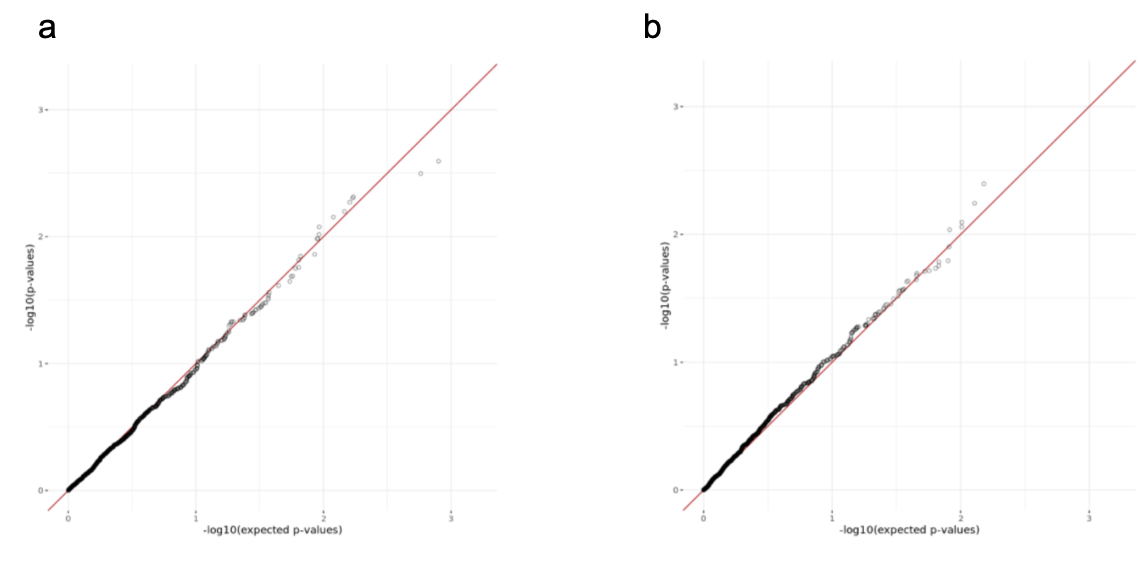
\includegraphics[width=15.5cm]{Chapter6/Fig/sc_structlmm_calibration.png}
\caption[qq plots]{\textbf{qq plots}.\\
calibration.}
\label{fig:sc_structlmm_calibration}
\end{figure}

% \subsection{Comparison with Struct LMM v0}

% Next, we compared our model to the original StructLMM model.
% StructLMM is expected to have issues in the presence of extended repeated structure, which it is not equipped to deal with.
% To address this, we simulated various numbers of repeats per donor - mimicking cells -  ranging from 10 to 500.
% Indeed, we observe over-inflation of StructLMM in the presence of many repeats making the model not calibrated (Fig. Xa).
% sc-StructLMM, on the other hand, is nicely calibrated (Fig. Xb).

% \subsection{Comparison with standard interaction test}

% We then performed power analysis when comparing our model with one where the environments are modelled as fixed effects (see Section 2.4.2).

\clearpage

% \section{Real data}
\section{Application to differentiating iPS cells}

We applied the model on the data described in Chapter 4.
% We applied our model on a recently published dataset \cite{cuomo2020single}. 
Here, cells from 125 donors are differentiated from a pluripotent state, to definitive endoderm. 
We use 
principal components (PCs) 
% 10 MOFA factors estimated from the data \cite{argelaguet2018multi}
% 500 independent ($r^2<0.2$) highly variable genes (HVGs)
to capture various aspects of the variation in gene expression in the dataset, which represent cell states and types. 
In particular, PC1 nicely aligns with the differentiation axis. 
We observe an increase in our power to identify interaction eGenes (genes with at least one interaction eQTL) as we increase the number of PCs used as environments, with then a plateau at 50 PCs (Fig.X).
Reassuringly, we can recapitulate most (XX\%) of the dynamic eQTL described in the original paper, which were detected using solely PC1, and a fixed effect linear mixed model (Methods). 
However, we show that we have increased power using our model. 
Furthermore, the overlap with our interaction eQTL and the dynamic eQTL identified in Cuomo \textit{et al}. decreases, the more PCs we include (Fig. XX).\\

\begin{figure}[htbp]
\centering
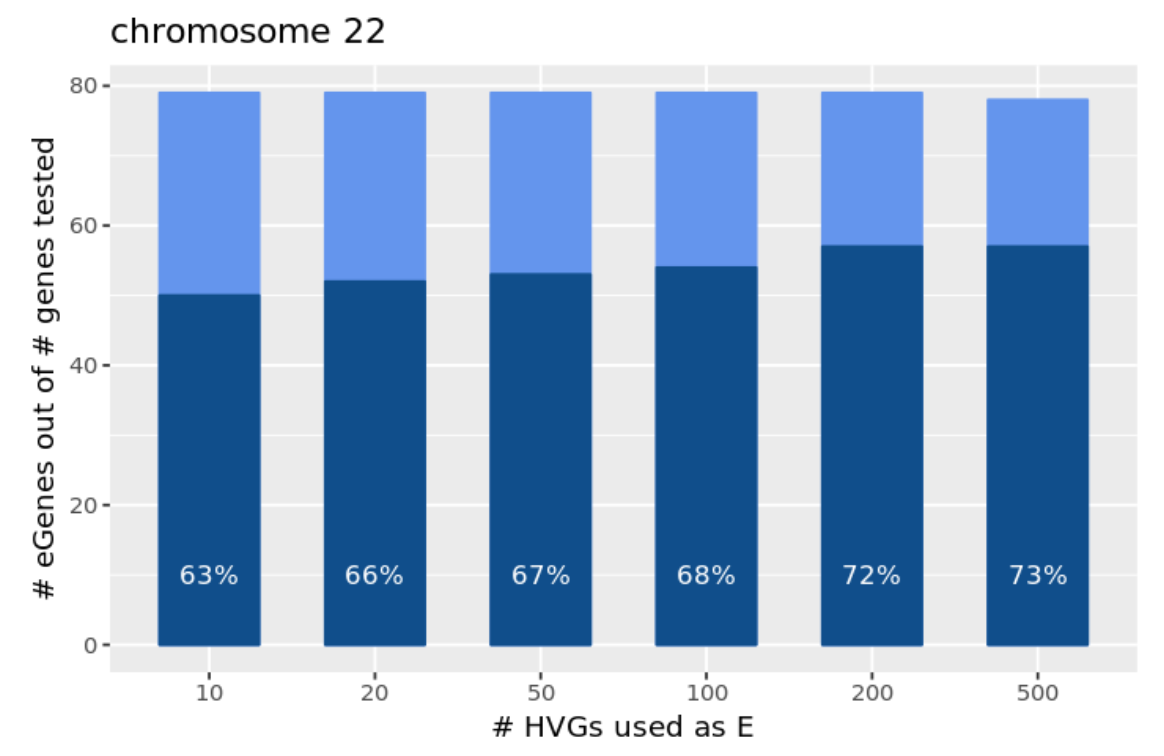
\includegraphics[width=15.5cm]{Chapter6/Fig/sc_structlmm_endodiff.png}
\caption[results on endodiff]{\textbf{results on endodiff}.\\
Barplots.}
\label{fig:sc_structlmm_endo_barplots}
\end{figure}

% As environments, we used
% the first 10 principal components


% PCs, MOFA, HVGs?
% transformation?
% normalization/scaling




% \section{Upstream analysis}

% One of the key steps in running this method is choosing the environmental factors.
% We expect most applications to be for scRNA-seq datasets only (and genotypes).
% This means that the environments need to be estimated from the transcriptomic data, which is also used as phenotype, causing concerns of circularity.


% A user might have 
% PCA
% MOFA (single omic)

% \section{Downstream analysis} 

% \subsection{Estimate cell-specific genetic effects}

\clearpage

\section{Predicting cell-specific effect sizes driven by GxE}

Using our model it is possible to estimate a cell-specific genetic effect size due to GxE (thus estimating $\boldsymbol{\beta_{GxE}}$) for each gene-SNP pair tested.

To do so, we...
 

\begin{equation}
    \mathbf{f}(\mathbf{X}) \sim \mathrm{GP}(\mathbf{m}(\mathbf{x}), k(\mathbf{x},\mathbf{x}^T))
\end{equation}

Out of sample prediction for $\mathbf{f}_*$'s best estimator is its best linear unbiased predictor (BLUP), defined as its expected value condition on $\mathbf{f}$ and $\mathbf{X},\mathbf{X}_*$:

\begin{equation}
    E[\mathbf{f}_*|\mathbf{f}] = \mathbf{m}_* +k(\mathbf{X}_*,\mathbf{X})k(\mathbf{X},\mathbf{X})^{-1}(\mathbf{f}-\mathbf{m})
\end{equation}

In our case,

\begin{equation}
    \mathbf{f}(\mathbf{X}) = \mathbf{y} = \mathbf{W}\boldsymbol{\alpha}+\mathbf{g}\beta_G+\mathbf{g}\boldsymbol{\beta}_{GxE}+\mathbf{e} + \mathbf{u} + \boldsymbol{\psi}
\end{equation}

with ($\mathbf{X} = {\mathbf{W},\mathbf{g},\mathbf{E},\mathbf{K}}$):

\begin{equation}
    \mathbf{m}(\mathbf{X}) = \mathbf{W}_*\boldsymbol{\alpha}_{*}+\mathbf{g}_*\beta_G
\end{equation}

\begin{equation}
    k(\mathbf{X},\mathbf{X}) = \sigma_{GxE}^2(\mathbf{g}\odot\mathbf{E})(\mathbf{g}\odot\mathbf{E})^T
\end{equation}

\begin{equation}
\mathbf{y}_{*}^{BLUP} = E[\mathbf{y}_*|\mathbf{y}] = 
\mathbf{W}_*\boldsymbol{\alpha}_{*}+\mathbf{g}_*\beta_G+\mathbf{E}_*\gamma + 
k(\mathbf{X}_*\mathbf{X})K^{-1}(\mathbf{y}-\mathbf{W}\boldsymbol{\alpha}-\mathbf{g}\beta_G-\mathbf{E}\gamma)
\end{equation}

We perform this analysis only for the subset of XXX eQTL that exhibit some GxE effects (FDR < 10\%).
Reassuringly, we see that Oct4, .. (Fig. \ref{fig:sc_structlmm_pcas}).\\

One important axis of variation is time, thus we cluster using Palantir \cite{setty2019characterization}
(Fig. \ref{fig:sc_structlmm_clusters}).

\begin{figure}[htbp]
\centering
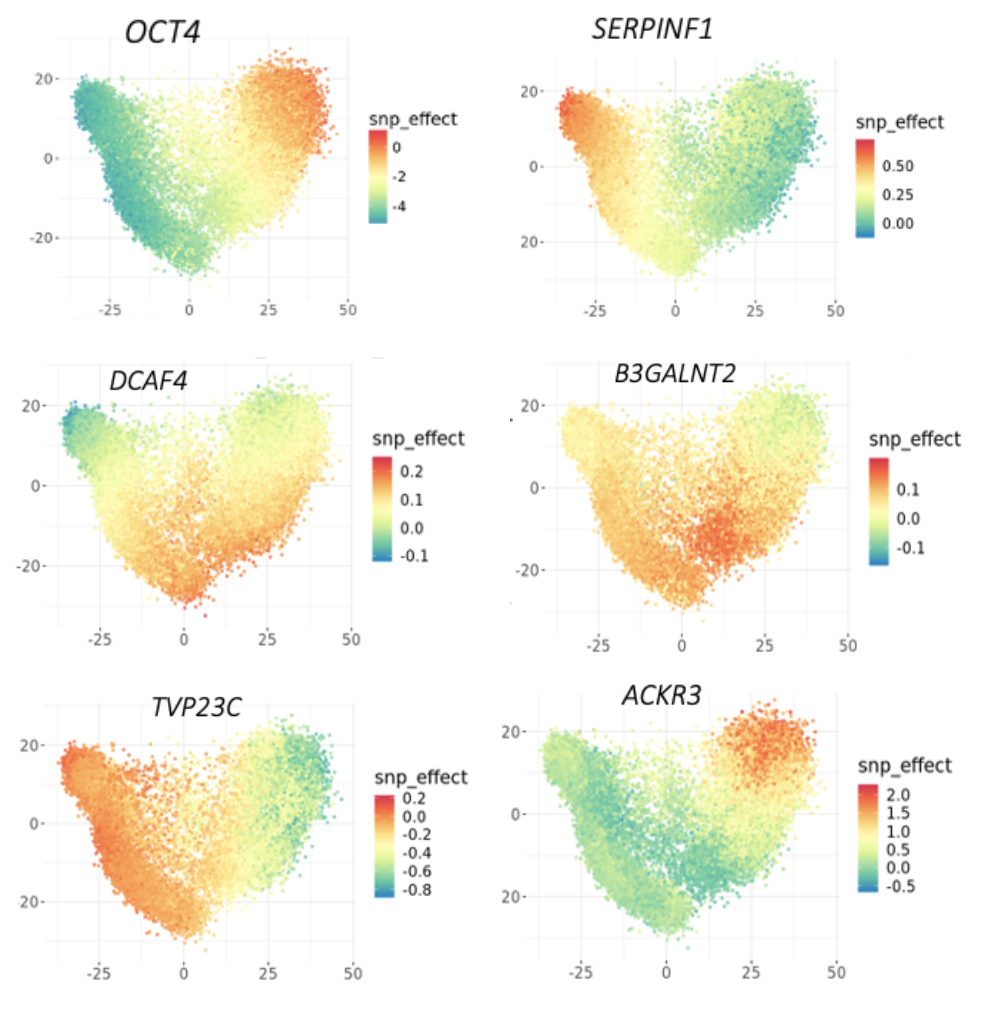
\includegraphics[width=15.5cm]{Chapter6/Fig/sc_structlmm_pcas.png}
\caption[cell-specific effect sizes]{\textbf{cell-specific effect sizes}.\\
PCA plots.}
\label{fig:sc_structlmm_pcas}
\end{figure}


\begin{figure}[h]
\centering
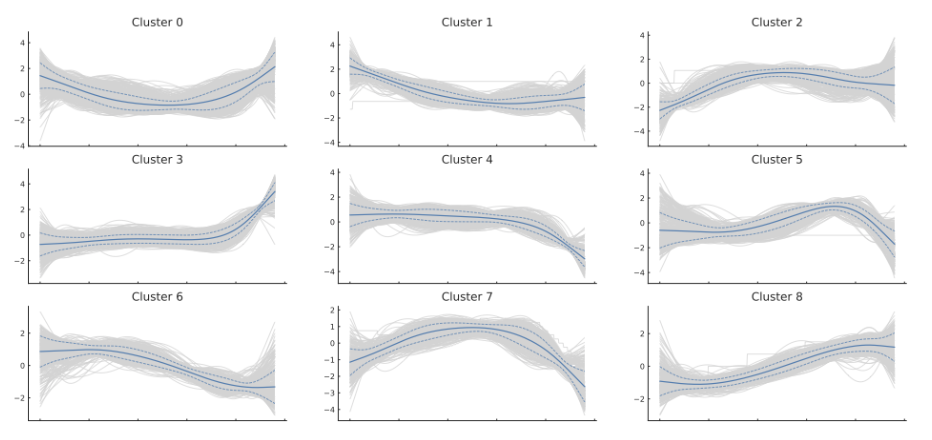
\includegraphics[width=15.5cm]{Chapter6/Fig/sc_structlmm_clusters.png}
\caption[clusters]{\textbf{clusters}.\\
Clusters using .}
\label{fig:sc_structlmm_clusters}
\end{figure}

\clearpage

\section{Discussion}

Here, I have presented a method that...

summarise and refer to figures\\

One of the key steps in running this method is choosing the environmental factors, prior to testing the method.
We expect most applications to be for scRNA-seq datasets only (and genotypes).
This means that the environments need to be estimated from the transcriptomic data, which is also used as phenotype, causing concerns of circularity.\\

On the other hand, downstream analysis steps may include methods to determine which of the included environments are responsible..\\

A limitation of the model is that it models the phenotype vector (single cell expression profile of a genes) as following a normal distribution.
We quantile-normalise y, which makes a difference, but future work should include extension to non-Gaussian likelihoods (e.g. Poisson, Negative Binomial).
However, GLMMs are slow..\\

Finally, while the main application of the method is single cell context-specific eQTL mapping across several states, this model is in principle flexible to any application with repeat measurements for the same individual (e.g. longitudinal data)
% \begin{itemize}
%     \item GLMM (Poisson, NB)
%     \item additional covariances?
%     \item other applications (longitudinal data)
% \end{itemize}
